\documentclass{article}

\usepackage{tikz}
\usetikzlibrary{shapes,arrows}
\begin{document}

\centering
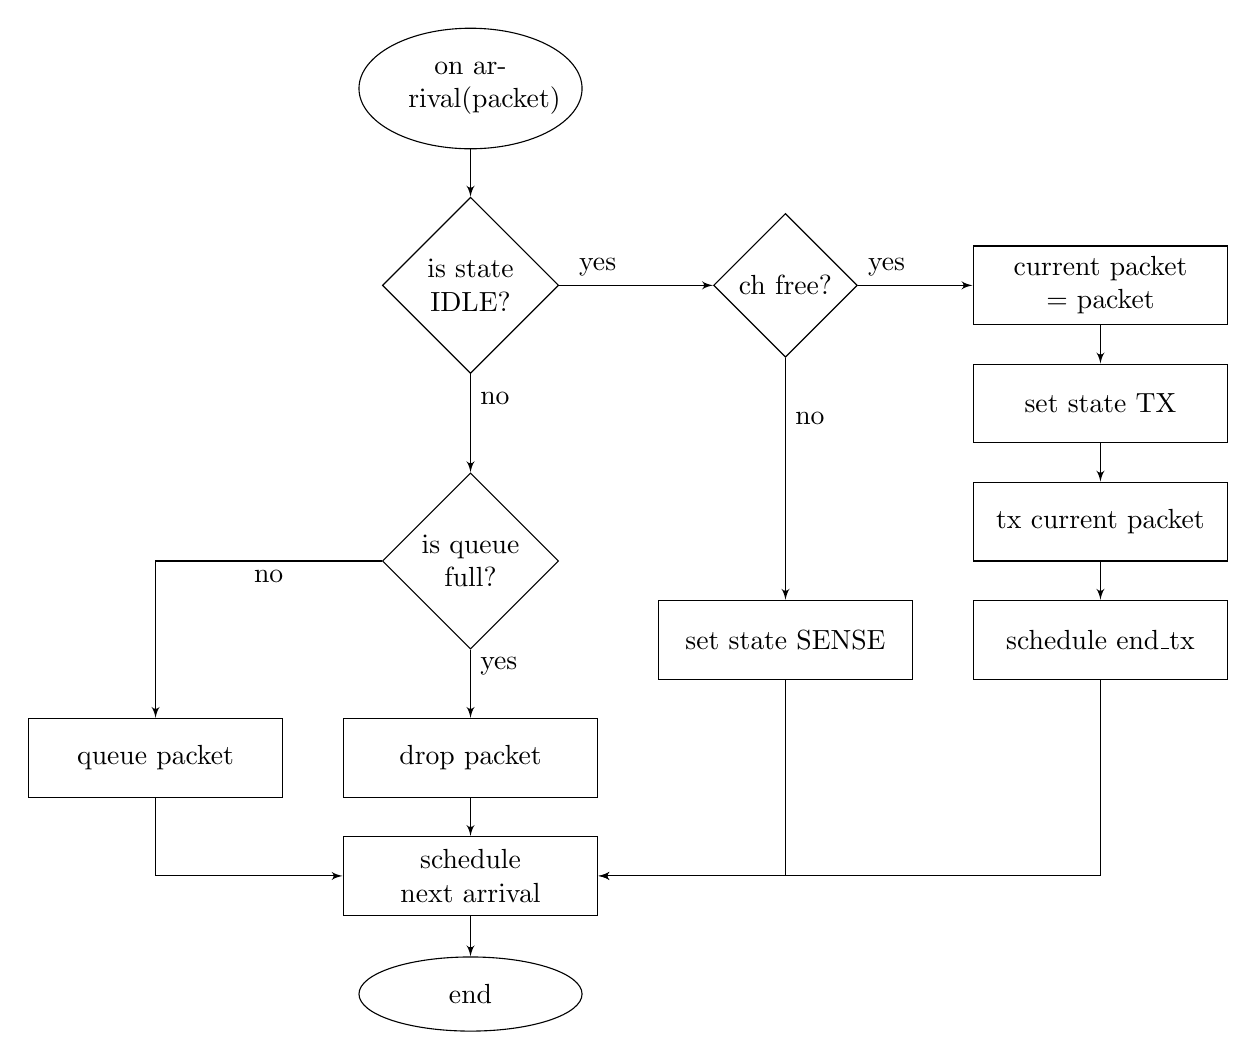
\begin{tikzpicture}[node distance = 1.5cm, auto]
    \tikzstyle{terminator} = [ellipse, draw,
    text width=4.5em, text centered, inner sep=6pt]
  \tikzstyle{decision} = [diamond, draw,
    text width=4.5em, text centered, node distance=3cm, inner sep=0pt]
  \tikzstyle{block} = [rectangle, draw, text width=3cm, text centered, minimum width=3cm,
    minimum height=1cm]
  \tikzstyle{line} = [draw, -latex']

  % Place nodes
  \node [terminator] (init) {on arrival(packet)};
  \node [decision, below of=init, node distance=2.5cm] (idle) {is state IDLE?};
  \node [decision, below of=idle, node distance=3.5cm] (queue) {is queue full?};
  \node [decision, right of=idle, node distance=4cm] (count) {ch free?};
    \node [block, right of=count, node distance=4cm] (curpk) {current
    packet = packet};
  \node [block, below of=curpk] (settx) {set state
    TX};
  \node [block, below of=settx] (tx) {tx current packet};
  \node [block, below of=tx] (sched_tx) {schedule end\_tx};
  \node [block, below of=count, node distance=4.5cm] (setsense) {set state SENSE};
  \node [block, below of=queue, node distance=2.5cm] (drop) {drop packet};
  \node [block, left of=drop, node distance=4cm] (enqueue) {queue packet};
  \node [block, below of=drop] (sched_arr) {schedule next arrival};
  \node [terminator, below of=sched_arr] (end) {end};

  % Draw edges
  \path [line] (init) -- (idle);
  \path [line] (idle) -- node [near start] {yes} (count);
  \path [line] (idle) -- node [near start] {no} (queue);
  \path [line] (queue) -- node [near start] {yes} (drop);
  \path [line] (queue) -| node [near start] {no} (enqueue);

  \path [line] (drop) -- (sched_arr);

  \path [line] (enqueue) |- (sched_arr);

  \path [line] (count) -- node [near start] {yes} (curpk);
  \path [line] (curpk) -- (settx);
  \path [line] (settx) -- (tx);
  \path [line] (tx) -- (sched_tx);
  \path [line] (sched_tx) |- (sched_arr);

  \path [line] (count) -- node [near start] {no} (setsense);
  \path [line] (setsense) |- (sched_arr);

  \path [line] (sched_arr) -- (end);
\end{tikzpicture}


\end{document}
